\chapter{Copulas and Its Applications}

Copulas (or copul\ae in Latin) are an interesting mathematical tool to represent correlations between probability distributions. They can be used to describe complex dependencies in multivariate risk models, when more basic tools such as a multivariate Gaussian distribution is inappropriate. Another commonly used application of copulas is sampling from correlated random variables.

In this Chapter the copula concept is reviewed and some example applications are shown. 
%Before going into the copulas we need to learn how to transform a distribution into another using the \emph{probability integral transform}. 

\section{Default Correlation}\label{sec:default_correlation}
Correlation is a precise mathematical concept that has only meaning in reference to random variables. If $X$ and $Y$ are random variables, the \emph{correlation coefficient}, $\rho$, between $X$ and $Y$ is defined as
\begin{equation}
\rho = \cfrac{\mathbb{E}[(X-\mu_Y)(Y-\mu_Y)]}{\sigma_X \sigma_Y}
\label{eq:correlation_coefficient}
\end{equation}
where $\mu$ and $\sigma$ denote mean and standard deviation of each random variable, while $\mathbb{E}$ is the expected value operator.

Thus, statements such as company $A$ and company $B$ are correlated are meaningless. One needs to refer to a quantifiable variable associated with the two companies (e.g. stock price, revenue growth or credit default spread) for that statement to make sense.
In the same spirit, stating that the default behavior of companies $A$ and $B$ is correlated does not carry a lot of meaning unless one specifies a random variable that captures what \emph{default behavior} means. %In summary, before
%we can talk about default correlation, we need to define a random variable
%that somehow captures \emph{default behavior}.

Consider two assets. Two random variables $P_1$ and $P_2$, i.e. the default probabilities, can be used to generate default scenarios for each asset. If $n$ of such possible default scenario are generated two index variables $v_1$ and $v_2$ capture the default pattern of each asset: each variable, actually a vector, will be a sequence of $n$ 1’s and 0’s according to the default state of the corresponding asset.

Using an appropriate random sample it is possible to determine the correlation coefficient between $v_1$ and $v_2$ to then estimate the default correlation ($\rho_D$) between asset 1 and 2.

\begin{equation}
\rho_D = \cfrac{n\sum (v_{1i} v_{2i}) - \sum v_{1i} \sum v_{2i}}{\sqrt{(n\sum v_{1i}^2 - (\sum v_{1i})^2)(n\sum w_{2i}^2 - (\sum w_{2i})^2)}}
\label{eq:discrete_correlation_coefficient}
\end{equation}
Equation~\ref{eq:discrete_correlation_coefficient} is just a discrete version of Eq.~\ref{eq:correlation_coefficient}.

The challenge to do a Monte Carlo relies on the modeler’s ability to generate
realistic default scenarios. That is, being able to be loyal to $p$ (the average
default probability of the pool) and $\rho_D$ (the assets’ default correlation.) Note that if we are dealing with two assets, the default correlation is captured by one number. In the case of $N$ assets, $\rho_D$ is a symmetric matrix. In the
simplest case, that is, when all the pair-wise correlations are the same, all the
off-diagonals elements are identical. 

\section{Distribution Transformation}\label{distribution-transformation}

Distribution transformation is a very useful tool which will be
extensively used with the copula concept that we discuss in the next
Sections. The technique we are going to outline transforms every random
variable, regardless its distribution, into uniform and vice versa and is called
\emph{inverse transform} or (probability integral transform).

Computationally, this method involves computing the quantile function 
(see Section~\ref{quantile-function}) of
the original distribution; in other words, computing the cumulative
distribution function ($F_X(x)$) (which maps a number
to a probability between 0 and 1) and then inverting that
function. 

\begin{attention}
\subsubsection{Demonstration}
Let's start with a random variable $X$ with an arbitrary distribution and let $F_X$ be the 
cumulative distribution function of $X$ (\(F(x) = P(X \leq x)\)).
We would like to find a transformation $T:[0,1]\rightarrow\mathbb{R}$ such that $T(U)=X$, where
$U$ is the uniform distribution in $[0,1]$. 
\begin{equation*}
F_{X}(x)= P(X\leq x)=P(T(U)\leq x)= P(U\leq T^{-1}(x))=T^{-1}(x),{\text{ for }}x\in \mathbb {R}
\end{equation*}
where the last step used that $P(U\leq y)=y$ when $U$ is uniform on $(0,1)$.

So we got $F_{X}$ to be the inverse function of $T$, or, equivalently $T(u)=F_{X}^{-1}(u)$, $u\in [0,1]$.
\end{attention}

Therefore to transform a generic random variable to uniform (and vice versa) we can use
\begin{equation}
x = F_{X}^{-1}(u)\quad\mathrm{and}\quad u = F_X(x)	
\end{equation} 

Let's see few examples of how this can be done in \(\tt{python}\).
Imagine we want to transform an uniform distribution into a Gaussian.
The transformation takes uniform samples of a variable \(u\) between 0 and
1, interpreted as a probability, and then returns $F^{-1}(u)$. 

Table~\ref{tab:transformation} shows the samples of $U$ and their representation on the standard normal
distribution determined using the algorithm explained above.

\begin{codebox}
\begin{Verbatim}[commandchars=\\\{\}]
\PY{k+kn}{from} \PY{n+nn}{scipy}\PY{n+nn}{.}\PY{n+nn}{stats} \PY{k}{import} \PY{n}{uniform}\PY{p}{,} \PY{n}{norm}
		
\PY{n}{uniform\PYZus{}samples} \PY{o}{=} \PY{p}{[}\PY{l+m+mf}{0.5}\PY{p}{,} \PY{o}{.}\PY{l+m+mi}{975}\PY{p}{,} \PY{l+m+mf}{0.995}\PY{p}{,} \PY{l+m+mf}{0.999999}\PY{p}{]}
\PY{k}{for} \PY{n}{u} \PY{o+ow}{in} \PY{n}{uniform\PYZus{}samples}\PY{p}{:}
    \PY{n+nb}{print} \PY{p}{(}\PY{n}{norm}\PY{o}{.}\PY{n}{ppf}\PY{p}{(}\PY{n}{u}\PY{p}{)}\PY{p}{)}
\end{Verbatim}
\end{codebox}

\begin{table}[h]
  \centering
  \begin{tabular}{|c|c|}
    \hline
    \(\mathbf{u}\) & \(\mathbf{F^{-1}(u)}\) \\
    \hline
    0.5 & 0 \\
    \hline
    .975 & 1.95996 \\
    \hline
    .995 & 2.5758 \\
    \hline
    .999999 & 4.75342 \\
    \hline
    \(1-2^{-52}\) & 8.12589 \\
    \hline
  \end{tabular}
  \caption{Table of samples from the uniform distribution and their corresponding Gaussian quantiles.}
\label{tab:transformation}
\end{table}

Now let's see how this can be done directly with an entire distribution. Let's start again from 
the uniform distribution. This can be sampled either using \texttt{random.random} 
like in Section~\ref{pseudo-random-numbers} or with \texttt{scipy.stats.uniform}. 
Each distribution defined in \texttt{scipy.stats} has a convenient method \texttt{rvs(size=aSize)} 
(random variable sample) to sample from it as many time as specified by the arguments \texttt{size}. 
Usually the second method is preferred since it exploits \texttt{numpy.array} and let us avoid a 
lot of for-loop cycles.

In any case in the left plot of Fig.~\ref{fig:uniform_and_gauss} the resulting distribution is shown.

\begin{codebox}
\begin{Verbatim}[commandchars=\\\{\}]
\PY{n}{x} \PY{o}{=} \PY{n}{uniform}\PY{p}{(}\PY{l+m+mi}{0}\PY{p}{,} \PY{l+m+mi}{1}\PY{p}{)}\PY{o}{.}\PY{n}{rvs}\PY{p}{(}\PY{l+m+mi}{10000}\PY{p}{)}
\end{Verbatim}
\end{codebox}

Next we want to transform these samples so that instead of uniform they
are normally distributed. As we have just seen the transform that does this
is the inverse of the cumulative density function of the normal 
distribution, or \((\tt{ppf(x))}\) in \texttt{python}. 

In the right plot of Fig.~\ref{fig:uniform_and_gauss} the Gaussian obtained 
with the code below is shown

\begin{codebox}
\begin{Verbatim}[commandchars=\\\{\}]
\PY{n}{x\PYZus{}trans} \PY{o}{=} \PY{n}{norm}\PY{o}{.}\PY{n}{ppf}\PY{p}{(}\PY{n}{x}\PY{p}{)}
\end{Verbatim}
\end{codebox}

\begin{figure}[htb]
	\centering
	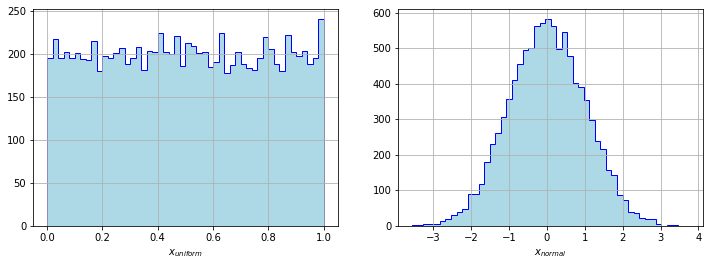
\includegraphics[width=1.\textwidth]{figures/uniform_gauss.png}
	\caption{On the left the generated uniform distribution, on the right its Gaussian transform.}
	\label{fig:uniform_and_gauss}
\end{figure}

If we plot them together in a 2D plot we can get a sense of what is
going on using the inverse CDF transformation.
Indeed it stretches the outer regions of the uniform to yield a
normal distribution. This is shown in Fig.~\ref{fig:uniform_to_gauss}. 
    
\begin{figure}[htbp]
  \centering
  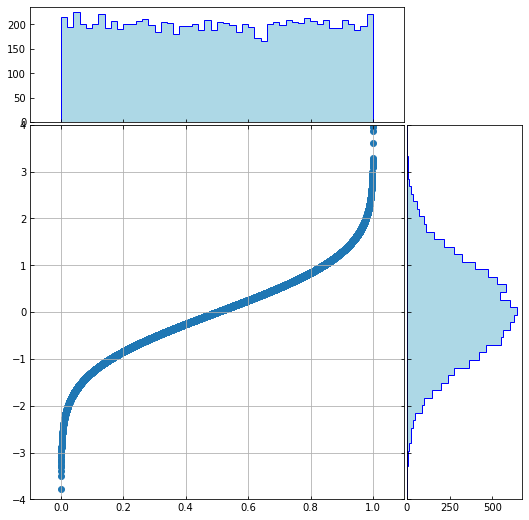
\includegraphics[width=0.5\textwidth]{figures/lesson6_7_0.png}
  \caption{2D plot showing the transformation that maps our initial uniform distribution to the resulting Gaussian.}
  \label{fig:uniform_to_gauss}
\end{figure}
    
The nice thing of this technique is that it can be used
for any arbitrary (univariate) probability distribution, like for
example t-Student~\cite{bib:t_student} or Gumbel~\cite{bib:gumbel}.
A similar transformation from uniform to t-Student is shown in Fig.~\ref{fig:uniform_to_tstudent}.

\begin{codebox}
\begin{Verbatim}[commandchars=\\\{\}]
\PY{k+kn}{from} \PY{n+nn}{scipy}\PY{n+nn}{.}\PY{n+nn}{stats} \PY{k}{import} \PY{n}{t}

\PY{n}{x\PYZus{}trans} \PY{o}{=} \PY{n}{t}\PY{p}{(4}\PY{p}{)}\PY{o}{.}\PY{n}{ppf}\PY{p}{(}\PY{n}{x}\PY{p}{)}
\end{Verbatim}
\end{codebox}

\begin{figure}[htb]
  \centering
  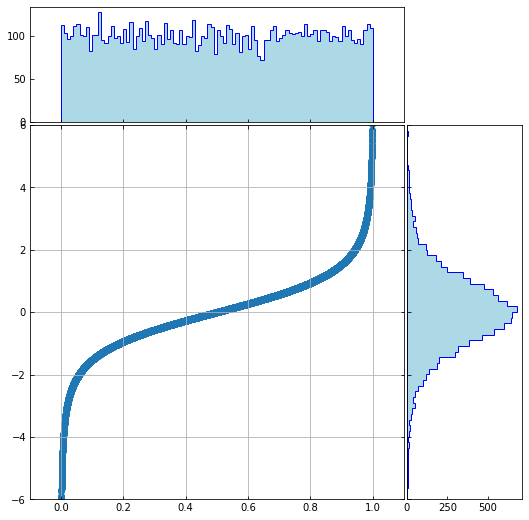
\includegraphics[width=0.5\textwidth]{figures/tstudent_to_uniform}
  \caption{2D plot showing the transformation that maps a uniform distribution to a t-Student.}
  \label{fig:uniform_to_tstudent}
\end{figure}

Clearly to do the opposite transformation, that is from an arbitrary distribution
to the uniform, we can just apply the inverse of the inverse CDF, that is the CDF itself\ldots

In such a way we can go from distribution A to distribution B passing through 
a uniform distribution rather quickly. An example is shown in Fig.~\ref{fig:a_to_b_to_a}.

\begin{figure}[htbp]
	\centering
	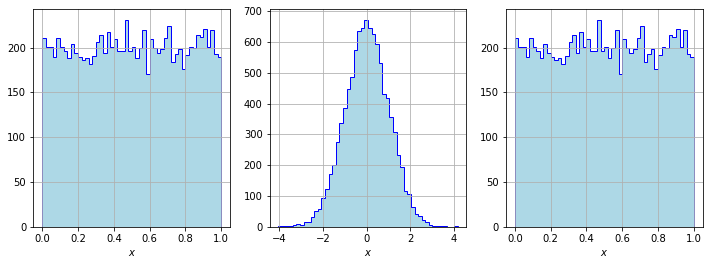
\includegraphics[width=1.\textwidth]{figures/a_to_b_to_a}
	\caption{Example of transformation, it starts with a uniform distribution, 
		goes into a Gaussian and back to the initial uniform.}
	\label{fig:a_to_b_to_a}
\end{figure}

\section{Copula}\label{copula}

In probability theory a \emph{copula} $\mathcal{C}(F_1, F_2, \ldots, F_n, \rho)$
is a multivariate (multidimensional) cumulative distribution function
whose marginal probability distributions (i.e. the probability
distribution of each dimension) are uniform on the
interval $[0, 1]$ ($F_i = U_i =\mathrm{uniform}(0,1)$),
\(\rho\) represents the correlation between each variable.

Copulas are used to describe the dependencies between random variables and
have been widely used in quantitative finance to model risk. Copulas are popular since
they allow to easily model and estimate the distribution of random
vectors by representing marginals and their correlation separately.

Essentially we can split a complicated problem into simpler components so that 
copula results to be very handy.

Despite the obscure and daunting definition given above the concept of copula is
quite simple so let's try to clarify it a bit with a practical example.

\subsection{Example Case}
\label{example-problem-case}

Imagine to have to measure two correlated variables. 
For example, we look at various rivers and for every river
at the maximum water level of that river over a certain
time-period. In addition, we also count how many months each river
caused floods.

For the probability distribution of the maximum level of the river we
know that maximums are Gumbel~\cite{bib:gumbel} distributed, 
while the number of floods
can be modeled according to a Beta~\cite{bib:eta}.

Clearly it is pretty reasonable to assume that maximum water level and
number of floods are going to be correlated, however we don't know how
we could model the correlated probability distribution.
Indeed above we only specified the distributions for individual variables, irrespective of the other one (i.e. the marginals), but in reality 
we are dealing with a \emph{joint distribution} of both of these together.
And here is where copulas come to our rescue.

Copulas essentially allow to decompose a joint probability distribution
into its marginals (which by definition have no correlation) and a
function which \textbf{couples} them together 
specifying the correlation separately. The copula is just that coupling
function.

\subsection{Adding Correlation with Gaussian Copulas}
\label{adding-correlation-with-gaussian-copulas}

How does this help us with our problem of creating a custom joint
probability distribution for maximum water level and floods ?

At the beginning of this Chapter we have seen how to convert anything
uniformly distributed to an arbitrary probability distribution, so we
could
\begin{itemize}
\tightlist
\item
  simulate a sample from a multivariate distribution with the specific correlation structure;
\item
  transform so that the marginals are uniform;
\item
  finally transform the uniform marginals to whatever we need to.
\end{itemize}

In this example we sample from a multivariate (two-dimensional) normal with a 0.5 correlation, 
see Fig.~ \ref{fig:multivariate_with_correlation}. This is not mandatory 
though, since
we could have modeled correlations with different distribution either.

\begin{codebox}
\begin{Verbatim}[commandchars=\\\{\}]
\PY{k+kn}{from} \PY{n+nn}{scipy}\PY{n+nn}{.}\PY{n+nn}{stats} \PY{k}{import} \PY{n}{multivariate_normal}

\PY{n}{mvnorm} \PY{o}{=} \PY{n}{multivariate\PYZus{}normal}\PY{p}{(}\PY{n}{mean}\PY{o}{=}\PY{p}{[}\PY{l+m+mi}{0}\PY{p}{,} \PY{l+m+mi}{0}\PY{p}{]} \PY{p}{,} \PY{n}{cov}\PY{o}{=}\PY{p}{[}\PY{p}{[}\PY{l+m+mi}{1}\PY{p}{,} \PY{l+m+mf}{0.5}\PY{p}{]}\PY{p}{,} \PY{p}{[}\PY{l+m+mf}{0.5}\PY{p}{,} \PY{l+m+mi}{1}\PY{p}{]}\PY{p}{]}\PY{p}{)}
\PY{n}{x} \PY{o}{=} \PY{n}{mvnorm}\PY{o}{.}\PY{n}{rvs}\PY{p}{(}\PY{l+m+mi}{100000}\PY{p}{)}
\end{Verbatim}
\end{codebox}

\begin{figure}[hb]
  \centering
  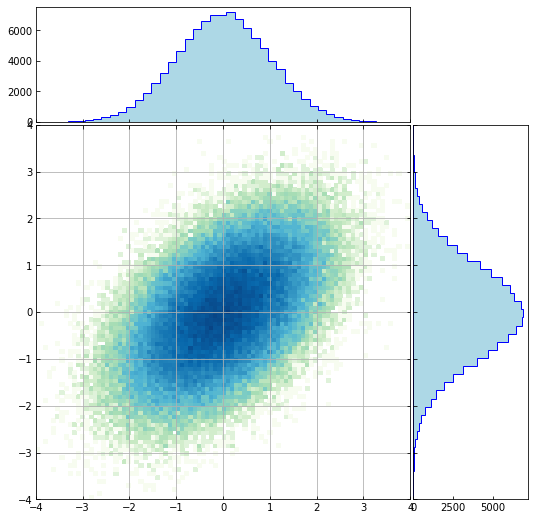
\includegraphics[width=0.5\textwidth]{figures/lesson6_14_0.png}
  \caption{2D normal distribution with a correlation factor of 0.5.}
  \label{fig:multivariate_with_correlation}
\end{figure}
    
Now use what we have just learned to make the marginals uniform using
the \(\tt{cdf}\) function of the normal distribution:

\begin{codebox}
\begin{Verbatim}[commandchars=\\\{\}]
\PY{n}{x\PYZus{}unif} \PY{o}{=} \PY{n}{norm}\PY{o}{.}\PY{n}{cdf}\PY{p}{(}\PY{n}{x}\PY{p}{)}
\end{Verbatim}
\end{codebox}

Plots like the one shown in Fig.~\ref{fig:copula} are how copulas are usually visualized. Since we have used a multivariate standard normal 
to model the correlation this is an example of \textbf{Gaussian Copula}.

\begin{figure}[htb]
\centering
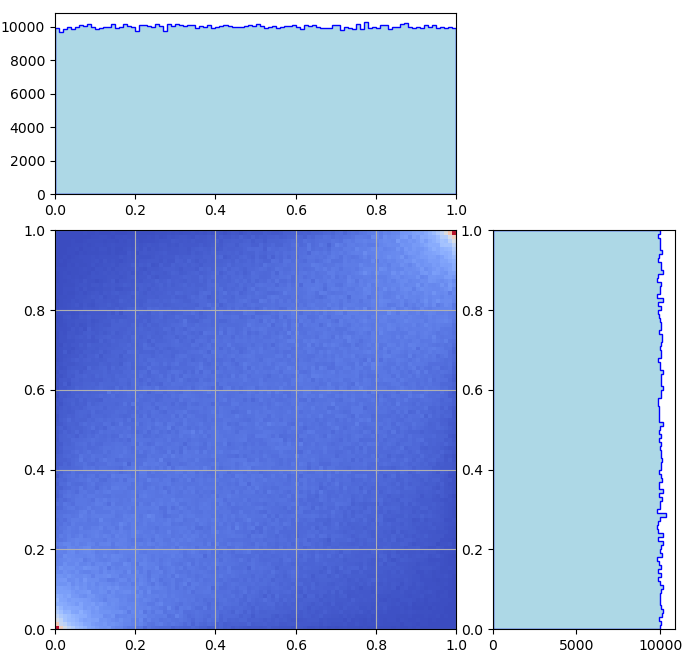
\includegraphics[width=0.45\textwidth]{figures/copula_2d}
\quad
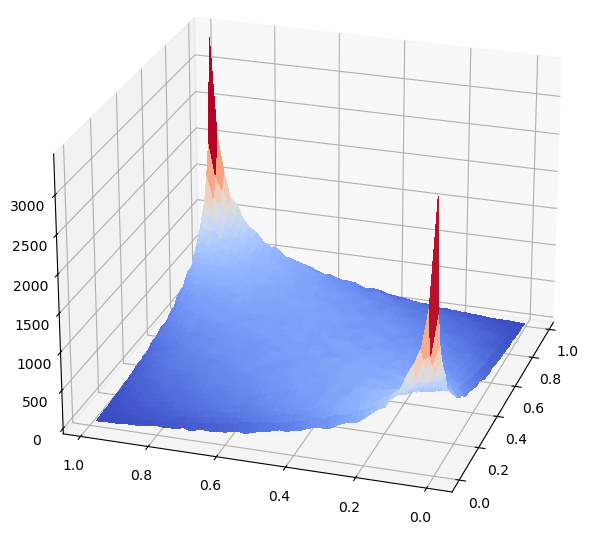
\includegraphics[width=0.5\textwidth]{figures/copula_3d}
\caption{Graphical representations of the copula, 2D on the left, 3D on the right.}
\label{fig:copula}
\end{figure}

Finally we can just transform the obtained marginals, again through uniform, 
to what we want (i.e. Gumbel and Beta in our river example):

\begin{codebox}
\begin{Verbatim}[commandchars=\\\{\}]
\PY{k+kn}{from} \PY{n+nn}{scipy}\PY{n+nn}{.}\PY{n+nn}{stats} \PY{k}{import} \PY{n}{gumbel_l, beta}

\PY{n}{m1} \PY{o}{=} \PY{n}{gumbel\PYZus{}l}\PY{p}{(}\PY{p}{)}
\PY{n}{x1} \PY{o}{=} \PY{n}{m1}\PY{o}{.}\PY{n}{ppf}\PY{p}{(}\PY{n}{x_unif[\PY{l+m+mi}{:}][\PY{l+m+mi}{0}]}\PY{p}{)}

\PY{n}{m2} \PY{o}{=} \PY{n}{beta}\PY{p}{(}\PY{n}{a}\PY{o}{=}\PY{l+m+mi}{10}\PY{p}{,} \PY{n}{b}\PY{o}{=}\PY{l+m+mi}{3}\PY{p}{)}
\PY{n}{x2} \PY{o}{=} \PY{n}{m2}\PY{o}{.}\PY{n}{ppf}\PY{p}{(}\PY{n}{x_unif[\PY{l+m+mi}{:}][\PY{l+m+mi}{1}]}\PY{p}{)}
\end{Verbatim}
\end{codebox}

Left plot of Figure~\ref{fig:gumbel_beta_with_corr} shows the two marginals and the joint distribution.
    
To see that it is actually working as expected we should now compare the joint
distributions with and without correlation. 
Looking at Figure~\ref{fig:gumbel_beta_with_corr} the difference is quite clear.

\begin{codebox}
\begin{Verbatim}[commandchars=\\\{\}]
\PY{c+c1}{\PYZsh{} sample from Gumbel}
\PY{n}{x1} \PY{o}{=} \PY{n}{m1}\PY{o}{.}\PY{n}{rvs}\PY{p}{(}\PY{l+m+mi}{10000}\PY{p}{)}
\PY{c+c1}{\PYZsh{} sample from Beta}
\PY{n}{x2} \PY{o}{=} \PY{n}{m2}\PY{o}{.}\PY{n}{rvs}\PY{p}{(}\PY{l+m+mi}{10000}\PY{p}{)}
\end{Verbatim}
\end{codebox}

\begin{figure}[htbp]
  \centering
  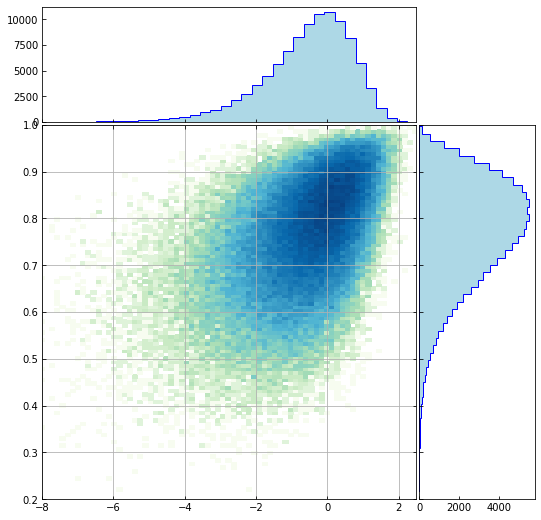
\includegraphics[width=0.45\textwidth]{figures/gumbel_vs_beta}
  \quad
  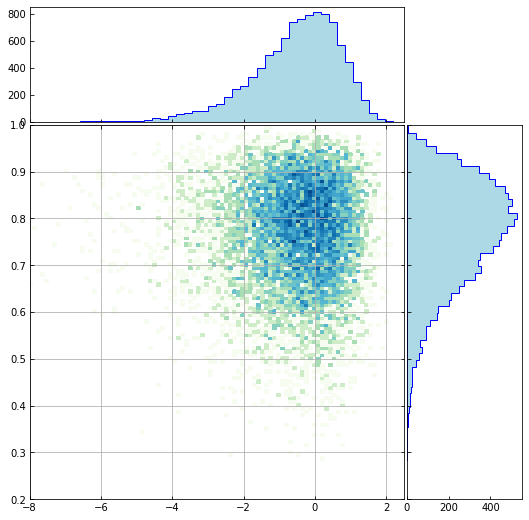
\includegraphics[width=0.45\textwidth]{figures/gumbel_vs_beta_corr}
  \caption{Marginalized Gumbel and Beta distributions with their joint when they is are (left) and are not (right) correlated.}
  \label{fig:gumbel_beta_with_corr}
\end{figure}
    
Using the uniform distribution as a common base for our transformations
we can easily introduce correlations and flexibly construct complex
probability distributions. 

As a final note, let's state \emph{Sklar's theorem} which assesses that any multivariate joint distribution can be written in terms of univariate marginal functions
and a copula which describes the dependence structure between the
variables.

Everything discussed in this Section can be easily generalized to higher dimensions.

%\subsection{Other Copulas}
%In the previous Section we have seen an application of a Gaussian copula but exists many other different 
%kind of copulas. Two typical examples are the t-copula and the Clayton copula.

%\subsubsection{t-copula}

%\subsubsection{Clayton copula}

\subsection{Generate Correlated Distributions}
\label{generate-correlated-distributions}

If we need to generate numbers from correlated distributions we can
follow similar steps to those described before:

\begin{itemize}
\tightlist
\item
  generate a random vector \(\mathbf{x}=(x_1, x_2,\ldots)\) from the
  original multivariate distribution with the desired correlation;
\item
  determine the single \(U_i(x_i)\) by applying \(\tt{cdf}\) to each
  \(x_i\);
\item
  transform again each \(U_i(x_i)\) to the desired marginal
  distributions using \(\tt{ppf}\);
\item
  each component of the vector \(\mathbf{x}\) is now converted to a set
  of random numbers drawn from the desired distributions, with the
  appropriate correlation.
\end{itemize}

A practical application concerns probability of default. 
Imagine three companies ($A$, $B$ and $C$) which have a
cumulative probability of defaulting within the next two years of 10\%.
Let's try to compute the probabilities to have the three of them all
defaulting within the next two years in two cases: independent default probabilities and perfectly correlated probabilities.

In the first case (independent probabilities), the
odds to get three defaults within two years will be the product
of the single probabilities, hence:

\[P_{\mathrm{uncorr}} = 10\% \cdot 10\% \cdot 10\% = 0.1 \%\]

We can verify this in \(\tt{python}\) by applying the method outlined above: first generate a random sample from an uncorrelated multivariate normal distribution, then transform each sampled vector into uniform with the \(\tt{norm.cdf}\) function (i.e. we
convert the sample into cumulative probabilities) and then count how many times the
three of them are lower than 10\% to check whether a default occurred in next two year (in this case, since we are interested in cumulative probabilities we can neglect the last transformation and work directly with the 
uniform marginals).

\begin{codebox}
\begin{Verbatim}[commandchars=\\\{\}]
\PY{k+kn}{from} \PY{n+nn}{scipy}\PY{n+nn}{.}\PY{n+nn}{stats} \PY{k}{import} \PY{n}{multivariate\PYZus{}normal}\PY{p}{,} \PY{n}{uniform}\PY{p}{,} \PY{n}{norm}
\PY{k+kn}{import} \PY{n+nn}{numpy}
	
\PY{n}{numpy}\PY{o}{.}\PY{n}{random}\PY{o}{.}\PY{n}{seed}\PY{p}{(}\PY{l+m+mi}{10}\PY{p}{)}
\PY{n}{trials} \PY{o}{=}\PY{l+m+mi}{10000}
\PY{n}{mvnorm\PYZus{}no\PYZus{}corr} \PY{o}{=} \PY{n}{multivariate\PYZus{}normal}\PY{p}{(}\PY{n}{mean}\PY{o}{=}\PY{p}{[}\PY{l+m+mi}{0}\PY{p}{,} \PY{l+m+mi}{0}\PY{p}{,} \PY{l+m+mi}{0}\PY{p}{]}\PY{p}{,} \PY{n}{cov}\PY{o}{=}\PY{p}{[}\PY{p}{[}\PY{l+m+mi}{1}\PY{p}{,} \PY{l+m+mi}{0}\PY{p}{,} \PY{l+m+mi}{0}\PY{p}{]}\PY{p}{,}
                                                          \PY{p}{[}\PY{l+m+mi}{0}\PY{p}{,} \PY{l+m+mi}{1}\PY{p}{,} \PY{l+m+mi}{0}\PY{p}{]}\PY{p}{,}
                                                          \PY{p}{[}\PY{l+m+mi}{0}\PY{p}{,} \PY{l+m+mi}{0}\PY{p}{,} \PY{l+m+mi}{1}\PY{p}{]}\PY{p}{]}\PY{p}{)}
\PY{n}{defaults} \PY{o}{=} \PY{l+m+mi}{0}
\PY{n}{x} \PY{o}{=} \PY{n}{mvnorm\PYZus{}no\PYZus{}corr}\PY{o}{.}\PY{n}{rvs}\PY{p}{(}\PY{n}{trials}\PY{p}{)}
\PY{n}{x\PYZus{}trans} \PY{o}{=} \PY{n}{norm}\PY{o}{.}\PY{n}{cdf}\PY{p}{(}\PY{n}{x}\PY{p}{)}
\PY{k}{for} \PY{n}{i} \PY{o+ow}{in} \PY{n+nb}{range}\PY{p}{(}\PY{n+nb}{len}\PY{p}{(}\PY{n}{x\PYZus{}trans}\PY{p}{)}\PY{p}{)}\PY{p}{:}
    \PY{k}{if} \PY{n}{x\PYZus{}trans}\PY{p}{[}\PY{n}{i}\PY{p}{]}\PY{p}{[}\PY{l+m+mi}{0}\PY{p}{]} \PY{o}{\PYZlt{}} \PY{l+m+mf}{0.1} \PY{o+ow}{and} \PY{n}{x\PYZus{}trans}\PY{p}{[}\PY{n}{i}\PY{p}{]}\PY{p}{[}\PY{l+m+mi}{1}\PY{p}{]} \PY{o}{\PYZlt{}} \PY{l+m+mf}{0.1} \PY{o+ow}{and} \PY{n}{x\PYZus{}trans}\PY{p}{[}\PY{n}{i}\PY{p}{]}\PY{p}{[}\PY{l+m+mi}{2}\PY{p}{]} \PY{o}{\PYZlt{}} \PY{l+m+mf}{0.1}\PY{p}{:}
	\PY{n}{defaults} \PY{o}{+}\PY{o}{=} \PY{l+m+mi}{1}
	
\PY{n+nb}{print} \PY{p}{(}\PY{l+s+s2}{\PYZdq{}}\PY{l+s+s2}{Defaults w/o correlation: }\PY{l+s+si}{\PYZob{}:.2f\PYZcb{}}\PY{l+s+s2}{\PYZpc{}}\PY{l+s+s2}{\PYZdq{}}\PY{o}{.}\PY{n}{format}\PY{p}{(}\PY{n}{defaults}\PY{o}{/}\PY{n}{trials}\PY{o}{*}\PY{l+m+mi}{100}\PY{p}{)}\PY{p}{)}

Defaults w/o correlation: 0.10\%
\end{Verbatim}
\end{codebox}
\noindent
The result is 0.1\% as expected.

If we repeat the same Monte Carlo experiment with perfectly correlated
default probabilities we have

\begin{codebox}
\begin{Verbatim}[commandchars=\\\{\}]
\PY{n}{mvnorm\PYZus{}corr} \PY{o}{=} \PY{n}{multivariate\PYZus{}normal}\PY{p}{(}\PY{n}{mean}\PY{o}{=}\PY{p}{[}\PY{l+m+mi}{0}\PY{p}{,}\PY{l+m+mi}{0}\PY{p}{,}\PY{l+m+mi}{0}\PY{p}{]}\PY{p}{,} \PY{n}{cov}\PY{o}{=}\PY{p}{[}\PY{p}{[}\PY{l+m+mi}{1}\PY{p}{,} \PY{l+m+mf}{0.999999}\PY{p}{,} \PY{l+m+mf}{0.999999}\PY{p}{]}\PY{p}{,}
                                                     \PY{p}{[}\PY{l+m+mf}{0.999999}\PY{p}{,} \PY{l+m+mi}{1}\PY{p}{,} \PY{l+m+mf}{0.999999}\PY{p}{]}\PY{p}{,}
                                                     \PY{p}{[}\PY{l+m+mf}{0.999999}\PY{p}{,} \PY{l+m+mf}{0.999999}\PY{p}{,} \PY{l+m+mi}{1}\PY{p}{]}\PY{p}{]}\PY{p}{)}
\PY{n}{defaults} \PY{o}{=} \PY{l+m+mi}{0}
\PY{n}{x} \PY{o}{=} \PY{n}{mvnorm\PYZus{}corr}\PY{o}{.}\PY{n}{rvs}\PY{p}{(}\PY{n}{trials}\PY{p}{)}
\PY{n}{x\PYZus{}trans} \PY{o}{=} \PY{n}{norm}\PY{o}{.}\PY{n}{cdf}\PY{p}{(}\PY{n}{x}\PY{p}{)}

\PY{k}{for} \PY{n}{v} \PY{o+ow}{in} \PY{n}{x\PYZus{}trans}\PY{p}{:}
    \PY{k}{if} \PY{n+nb}{max}\PY{p}{(}\PY{n}{v}\PY{p}{)} \PY{o}{\PYZlt{}} \PY{l+m+mf}{0.1}\PY{p}{:}
        \PY{n}{defaults} \PY{o}{+}\PY{o}{=} \PY{l+m+mi}{1}

\PY{n+nb}{print} \PY{p}{(}\PY{l+s+s2}{\PYZdq{}}\PY{l+s+s2}{Defaults w/ correlation: }\PY{l+s+si}{\PYZob{}:.2f\PYZcb{}}\PY{l+s+s2}{\PYZpc{}}\PY{l+s+s2}{\PYZdq{}}\PY{o}{.}\PY{n}{format}\PY{p}{(}\PY{n}{defaults}\PY{o}{/}\PY{n}{trials}\PY{o}{*}\PY{l+m+mi}{100}\PY{p}{)}\PY{p}{)}

Defaults w/ correlation: 9.89\%
\end{Verbatim}
\end{codebox}
In this case the result is close to 10\%, like we had only one single company
defaulting. 
Indeed given the perfect correlation between the probabilities either there is no default or three "simultaneous" defaults with 10\% probability.

%\subsubsection{Independent Defaults}\label{independent-defaults}
%
%If the default times of the number of companies are independent,
%default probabilities can be
%calculated through multiplication and integration of the single default
%probability curves without Monte Carlo simulation.
%
%As an example, consider the probability to have two defaults among four
%companies. Let \(\tau_i\) be the default time of name \(i\) and \(F_i(t)\)
%its distribution. Then the probability that name 1 defaults second in
%the basket before time \(t\) is:
%
%\begin{equation}
%\begin{split}
%&\mathbb{P}((\tau_2\lt\tau_1)\cap (\tau_1\lt t)\cap (\tau_1\lt\tau_3)\cap (\tau_1\lt\tau_4)) +\\
%&\mathbb{P}((\tau_3\lt\tau_1)\cap (\tau_1\lt t)\cap (\tau_1\lt\tau_2)\cap (\tau_1\lt\tau_4)) =\\
%&\int_0^t{F_2 (s)\cdot (1-F_3 (s)) \cdot (1-F_4 (s))~dF_1(s)} +  \int_0^t{F_3 (s)\cdot (1-F_2 (s)) \cdot (1-F_4 (s))~dF_1(s)}
%\end{split}
%\label{eq:indep_default}
%\end{equation}
%
%Suppose the default probabilities of three companies, $A$, $B$ and $C$ are
%given as in the following table (in each interval are linear):
%
%\begin{center}
%	\begin{tabular}{|c|c|c|c|}
%		\hline
%		time in years & A & B & C \\
%		\hline
%		\hline
%		0 & 0 & 0 & 0 \\
%		1 & 0.022032 & 0.0317 & 0.035 \\
%		2 & 0.046242 & 0.0655 & 0.075 \\
%		3 & 0.07266 & 0.1022 & 0.121 \\
%		4 & 0.101233 & 0.142 & 0.153 \\
%		5 & 0.131885 & 0.1752 & 0.205 \\
%		\hline
%	\end{tabular}
%\end{center}
%and suppose that the default events of the three companies are
%independent. The integral in Eq.~\ref{eq:indep_default} can be solved by substitution:
%
%\[ \int_{x_0}^{x_1}{(1-F_B(x))(1-F_C(x))dF_A(x)}\]
%
%Setting \(t=m_A x + q_A\) it becomes:
%
%\[ \int_{m_A x_0 + q_A}^{m_A x_1 + q_A}{(1-F_B(x(t)))(1-F_C(x(t)))dt}\qquad\Big(\textrm{with}~x(t) = \cfrac{t -q_A}{m_A}\Big) \]
%and similarly for company $B$ and $C$.
%
%To convert it into \texttt{python} we can use \texttt{scipy.integrate.quad} to
%perform the integral and \texttt{numpy.interp} to determine the
%intermediate default probabilities.
%
%\begin{codebox}
%	\begin{Verbatim}[commandchars=\\\{\}]
%	\PY{k+kn}{from} \PY{n+nn}{scipy}\PY{n+nn}{.}\PY{n+nn}{integrate} \PY{k}{import} \PY{n}{quad}
%	\PY{k+kn}{from} \PY{n+nn}{numpy} \PY{k}{import} \PY{n}{interp}
%	
%	\PY{n}{default\PYZus{}rates} \PY{o}{=} \PY{p}{\PYZob{}}\PY{l+s+s2}{\PYZdq{}}\PY{l+s+s2}{A}\PY{l+s+s2}{\PYZdq{}}\PY{p}{:}\PY{p}{(}\PY{l+m+mi}{0}\PY{p}{,} \PY{l+m+mf}{0.022032}\PY{p}{,} \PY{l+m+mf}{0.046242}\PY{p}{,} \PY{l+m+mf}{0.07266}\PY{p}{,} \PY{l+m+mf}{0.101233}\PY{p}{,} \PY{l+m+mf}{0.131885}\PY{p}{)}\PY{p}{,}
%	\PY{l+s+s2}{\PYZdq{}}\PY{l+s+s2}{B}\PY{l+s+s2}{\PYZdq{}}\PY{p}{:}\PY{p}{(}\PY{l+m+mi}{0}\PY{p}{,} \PY{l+m+mf}{0.0317}\PY{p}{,} \PY{l+m+mf}{0.0655}\PY{p}{,} \PY{l+m+mf}{0.1022}\PY{p}{,} \PY{l+m+mf}{0.142}\PY{p}{,} \PY{l+m+mf}{0.1752}\PY{p}{)}\PY{p}{,}
%	\PY{l+s+s2}{\PYZdq{}}\PY{l+s+s2}{C}\PY{l+s+s2}{\PYZdq{}}\PY{p}{:}\PY{p}{(}\PY{l+m+mi}{0}\PY{p}{,} \PY{l+m+mf}{0.035}\PY{p}{,} \PY{l+m+mf}{0.075}\PY{p}{,} \PY{l+m+mf}{0.121}\PY{p}{,} \PY{l+m+mf}{0.153}\PY{p}{,} \PY{l+m+mf}{0.205}\PY{p}{)}\PY{p}{\PYZcb{}}
%	
%	\PY{k}{def} \PY{n+nf}{func}\PY{p}{(}\PY{n}{x}\PY{p}{,} \PY{n}{default}\PY{p}{,} \PY{n}{companies}\PY{p}{,} \PY{n}{t}\PY{p}{)}\PY{p}{:}
%	\PY{n}{m} \PY{o}{=} \PY{n}{default}\PY{p}{[}\PY{n}{companies}\PY{p}{[}\PY{l+m+mi}{0}\PY{p}{]}\PY{p}{]}\PY{p}{[}\PY{n}{t}\PY{p}{]} \PY{o}{\PYZhy{}} \PY{n}{default}\PY{p}{[}\PY{n}{companies}\PY{p}{[}\PY{l+m+mi}{0}\PY{p}{]}\PY{p}{]}\PY{p}{[}\PY{n}{t}\PY{o}{\PYZhy{}}\PY{l+m+mi}{1}\PY{p}{]}
%	\PY{n}{q} \PY{o}{=} \PY{n}{default}\PY{p}{[}\PY{n}{companies}\PY{p}{[}\PY{l+m+mi}{0}\PY{p}{]}\PY{p}{]}\PY{p}{[}\PY{n}{t}\PY{o}{\PYZhy{}}\PY{l+m+mi}{1}\PY{p}{]} \PY{o}{\PYZhy{}} \PY{n}{m} \PY{o}{*} \PY{p}{(}\PY{n}{t}\PY{o}{\PYZhy{}}\PY{l+m+mi}{1}\PY{p}{)}
%	\PY{n}{t} \PY{o}{=} \PY{p}{(}\PY{n}{x}\PY{o}{\PYZhy{}}\PY{n}{q}\PY{p}{)}\PY{o}{/}\PY{n}{m}
%	\PY{n}{F2} \PY{o}{=} \PY{l+m+mi}{1} \PY{o}{\PYZhy{}} \PY{n}{interp}\PY{p}{(}\PY{n}{t}\PY{p}{,} \PY{n+nb}{range}\PY{p}{(}\PY{n+nb}{len}\PY{p}{(}\PY{n}{default}\PY{p}{[}\PY{n}{companies}\PY{p}{[}\PY{l+m+mi}{1}\PY{p}{]}\PY{p}{]}\PY{p}{)}\PY{p}{)}\PY{p}{,} \PY{n}{default}\PY{p}{[}\PY{n}{companies}\PY{p}{[}\PY{l+m+mi}{1}\PY{p}{]}\PY{p}{]}\PY{p}{)}
%	\PY{n}{F3} \PY{o}{=} \PY{l+m+mi}{1} \PY{o}{\PYZhy{}} \PY{n}{interp}\PY{p}{(}\PY{n}{t}\PY{p}{,} \PY{n+nb}{range}\PY{p}{(}\PY{n+nb}{len}\PY{p}{(}\PY{n}{default}\PY{p}{[}\PY{n}{companies}\PY{p}{[}\PY{l+m+mi}{2}\PY{p}{]}\PY{p}{]}\PY{p}{)}\PY{p}{)}\PY{p}{,} \PY{n}{default}\PY{p}{[}\PY{n}{companies}\PY{p}{[}\PY{l+m+mi}{2}\PY{p}{]}\PY{p}{]}\PY{p}{)}
%	\PY{k}{return} \PY{n}{F2}\PY{o}{*}\PY{n}{F3}
%	
%	\PY{k}{def} \PY{n+nf}{integral}\PY{p}{(}\PY{n}{default}\PY{p}{,} \PY{n}{companies}\PY{p}{,} \PY{n}{t}\PY{p}{)}\PY{p}{:}
%	\PY{k}{return} \PY{n}{quad}\PY{p}{(}\PY{n}{func}\PY{p}{,} \PY{l+m+mi}{0}\PY{p}{,} \PY{n}{default}\PY{p}{[}\PY{n}{companies}\PY{p}{[}\PY{l+m+mi}{0}\PY{p}{]}\PY{p}{]}\PY{p}{[}\PY{n}{t}\PY{p}{]}\PY{p}{,} 
%	
%	\PY{n}{args}\PY{o}{=}\PY{p}{(}\PY{n}{default}\PY{p}{,} \PY{n}{companies}\PY{p}{,} \PY{n}{t}\PY{p}{)}\PY{p}{)}\PY{p}{[}\PY{l+m+mi}{0}\PY{p}{]}
%	\PY{k}{for} \PY{n}{companies} \PY{o+ow}{in} \PY{p}{[}\PY{p}{(}\PY{l+s+s2}{\PYZdq{}}\PY{l+s+s2}{A}\PY{l+s+s2}{\PYZdq{}}\PY{p}{,} \PY{l+s+s2}{\PYZdq{}}\PY{l+s+s2}{B}\PY{l+s+s2}{\PYZdq{}}\PY{p}{,} \PY{l+s+s2}{\PYZdq{}}\PY{l+s+s2}{C}\PY{l+s+s2}{\PYZdq{}}\PY{p}{)}\PY{p}{,} \PY{p}{(}\PY{l+s+s2}{\PYZdq{}}\PY{l+s+s2}{B}\PY{l+s+s2}{\PYZdq{}}\PY{p}{,} \PY{l+s+s2}{\PYZdq{}}\PY{l+s+s2}{A}\PY{l+s+s2}{\PYZdq{}}\PY{p}{,} \PY{l+s+s2}{\PYZdq{}}\PY{l+s+s2}{C}\PY{l+s+s2}{\PYZdq{}}\PY{p}{)}\PY{p}{,} \PY{p}{(}\PY{l+s+s2}{\PYZdq{}}\PY{l+s+s2}{C}\PY{l+s+s2}{\PYZdq{}}\PY{p}{,} \PY{l+s+s2}{\PYZdq{}}\PY{l+s+s2}{A}\PY{l+s+s2}{\PYZdq{}}\PY{p}{,} \PY{l+s+s2}{\PYZdq{}}\PY{l+s+s2}{B}\PY{l+s+s2}{\PYZdq{}}\PY{p}{)}\PY{p}{]}\PY{p}{:}
%	\PY{n}{prob} \PY{o}{=} \PY{l+m+mi}{0}
%	\PY{k}{for} \PY{n}{t} \PY{o+ow}{in} \PY{n+nb}{range}\PY{p}{(}\PY{l+m+mi}{1}\PY{p}{,} \PY{l+m+mi}{6}\PY{p}{)}\PY{p}{:}
%	\PY{n}{prob} \PY{o}{=} \PY{n}{integral}\PY{p}{(}\PY{n}{default\PYZus{}rates}\PY{p}{,} \PY{n}{companies}\PY{p}{,} \PY{n}{t}\PY{p}{)}
%	\PY{n+nb}{print} \PY{p}{(}\PY{l+s+s2}{\PYZdq{}}\PY{l+s+s2}{P(1st def) at time (}\PY{l+s+si}{\PYZob{}\PYZcb{}}\PY{l+s+s2}{) for company }\PY{l+s+si}{\PYZob{}\PYZcb{}}\PY{l+s+s2}{: }\PY{l+s+si}{\PYZob{}:.5f\PYZcb{}}\PY{l+s+s2}{\PYZdq{}}\PY{o}{.}\PY{n}{format}\PY{p}{(}\PY{n}{t}\PY{p}{,} 
%	\PY{n}{companies}\PY{p}{[}\PY{l+m+mi}{0}\PY{p}{]}\PY{p}{,} \PY{n}{prob}\PY{p}{)}\PY{p}{)}
%	
%	First to default prob at time (1) for company A: 0.02131
%	First to default prob at time (2) for company A: 0.04301
%	First to default prob at time (3) for company A: 0.06460
%	First to default prob at time (4) for company A: 0.08573
%	First to default prob at time (5) for company A: 0.10606
%	First to default prob at time (1) for company B: 0.03080
%	First to default prob at time (2) for company B: 0.06160
%	...
%	\end{Verbatim}
%\end{tcolorbox}

\section{Exercises}
\begin{question}
Using the \emph{probability integral transform} transform a Gumbel distribution into a Gaussian. Plot also all the distributions involved in the transformation.
\end{question}

\cprotEnv\begin{solution}
\begin{ipython}
from scipy.stats import gumbel_l, norm
from matplotlib import pyplot as plt

gumbel = gumbel_l()
xg = gumbel.rvs(100000)
xu = gumbel.cdf(xg)
xn = norm.ppf(xu)

sub1 = plt.subplot(1, 3, 1)
sub1.hist(xg, 50)
sub1.grid(True)
sub1.set_xlabel("$x_{gumbel}$")
sub2 = plt.subplot(1, 3, 2)
sub2.hist(xu, 50)
sub2.grid(True)
sub2.set_xlabel("$x_{uniform}$")
sub3 = plt.subplot(1, 3, 3)
sub3.hist(xn, 50)
sub3.grid(True)
sub3.set_xlabel("$x_{normal}$")
plt.show()
\end{ipython}

\begin{figure}[htbp]
\begin{center}
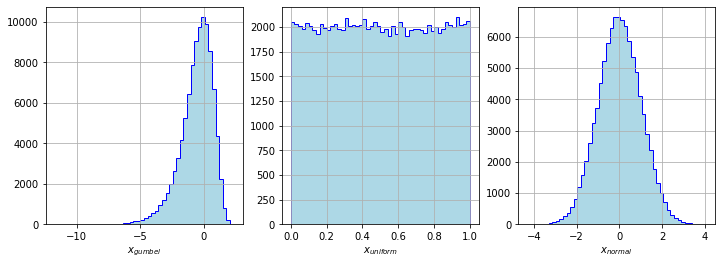
\includegraphics[width=0.9\linewidth]{figures/ex_gumbel_to_gauss.png}
\end{center}
\end{figure}
\end{solution}

\begin{question}
Without using the corresponding \texttt{rvs()} method try to generate 10 random numbers distributed as Beta distribution (parameters \texttt{a=3} and \texttt{b=10}).

\noindent\textbf{Hint:} starts with generating uniformly distributed random numbers.
\end{question}	

\cprotEnv\begin{solution}
\begin{ipython}
from scipy.stats import beta, uniform

x = uniform.rvs(size=10)
b = beta(a=3, b=10)
x_b = b.ppf(x)

print (x_b)
\end{ipython}
\begin{ioutput}
[0.29190237 0.45669406 0.10336582 0.5403107 0.08305872 0.32425694
0.43902811 0.11820592 0.28659784 0.22316621]
\end{ioutput}
\end{solution}

\begin{question}
Consider two companies whose default probabilities as a function of time are modeled according to a lognormal distribution with $\sigma =0.5$ (\texttt{scipy.stats.lognorm(0.5)}). Compare the joint 2D distributions in case of no correlation and with a Gaussian correlation of 0.8.

\noindent\textbf{Hint:} to plot the joint distribution use \texttt{matplotlib} function \texttt{hist2d(x1, x2, range=[[x1min, x1max], [xmin, x2max]], bins=(50, 50)) }.
\end{question}

\cprotEnv\begin{solution}
\begin{ipython}
from scipy.stats import lognorm, multivariate_normal, norm
import numpy

numpy.random.seed(1)
samples = 1000000
l1_uncorr = lognorm(0.5).rvs(size=samples)
l2_uncorr = lognorm(0.5).rvs(size=samples)
mvnorm = multivariate_normal(mean = (0, 0), 
                             cov = [[1, 0.8],
                                    [0.8, 1]])
x = mvnorm.rvs(size=samples)
x_corr = norm.cdf(x)
l1_corr = lognorm(0.5).ppf(x_corr[:, 0])
l2_corr = lognorm(0.5).ppf(
x_corr[:, 1])
plt.figure(figsize=(12, 4))
sub1 = plt.subplot(1, 2, 1)
sub1.hist2d(l1_uncorr, l2_uncorr, range=[[0, 2], [0, 2]], bins=(100, 100))
sub2 = plt.subplot(1, 2, 2)
sub2.hist2d(l1_corr, l2_corr, range=[[0, 2], [0, 2]], bins=(100, 100))
plt.show()
\end{ipython}
\noindent 
The resulting comparison is shown in Fig.~\ref{fig:joint_2d}.
\begin{figure}[htbp]
\begin{center}
	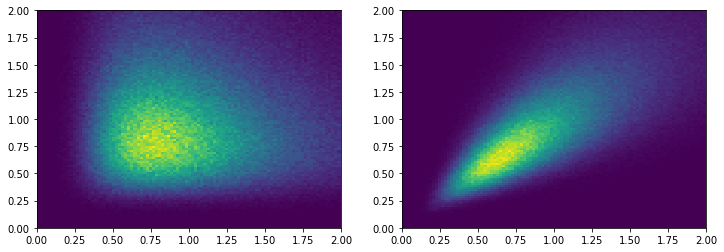
\includegraphics[width=0.9\linewidth]{figures/copula_lognormal.png}
\end{center}
\caption{Comparision of the joint 2D distributions in case of no correlation (left) and with a Gaussian correlation of 0.8 (right).}
\label{fig:joint_2d}
\end{figure}

In order to quantify the difference shown with the comparison of the two 2D plots we can calculate the probability that both companies default in the next six months.

So the probability that a single company default in six months regardless the other can be calculated from the \texttt{cdf} of the lognormal distribution.
Hence in case of independent probabilities what required is just the squared of this value (about 0.07\%).

\begin{ipython}
default_6m = lognorm(0.5).cdf(.5)
print(default_6m**2)
\end{ipython}
\begin{ioutput}
0.006860563560014724
\end{ioutput}

In the case of correlation instead we have to loop over the samples from the joint multivariate distribution (with correlation) and check how many times both values are less than \texttt{default\_6m}.

\begin{ipython}
success = 0.0
for i in range(samples):
    if max(x_corr[i]) < default_2:
        success += 1

print (success/samples)
\end{ipython}
\begin{ioutput}
0.044654
\end{ioutput}

This result can be interpreted graphically by saying that the entries in the "square" $[0, 0.5]$ in the left histogram are about 0.7\% of the total while the entries in the right plot in same "square" are about 4.5\% of the total. 
\end{solution}


\begin{thebibliography}{9}
\bibitem{bib:copula}P. Wilmott, \emph{Quantitative Finance (2nd edition)}, Credit Derivatives (Ch. 41), John Wiley and Sons, 2006 
\bibitem{bib:copula_nelsen}R. Nelsen, \emph{An Introduction to Copulas}, Springer–Verlag, 1999
\bibitem{bib:copula_cherubini}U. Cherubini, E. Luciano, W. Vecchiato, \emph{Copula Methods in Finance}, John Wiley \& Sons, 2004
\bibitem{bib:tstudent}\href{https://en.wikipedia.org/wiki/Student\%27s\_t-distribution}{\emph{t-Student distribution}}, Wikipedia [Online]
\bibitem{bib:Gumbel}\href{https://en.wikipedia.org/wiki/Gumbel_distribution}{\emph{Gumbel distribution}}, Wikipedia [Online]
\bibitem{bib:beta}\href{https://en.wikipedia.org/wiki/Beta_distribution}{\emph{Beta distribution}}, Wikipedia [Online]
\end{thebibliography}
